\section{Specification of Buddy Allocation Model}
The specification of the buddy memory allocation consists of a model for the necessary data structures to represent the memory layouts, as well as the allocation and disposal operations. This specification follows the algorithms for the buddy memory management in Zephyr OS, which applies a quartering split over blocks.

\subsection{State Representation}
\label{statedes}
The specification begins with the structure of a quad-tree.
{\footnotesize
\begin{align*}
&(set:\ 'a)\ tree\ =\ Leaf\ (L:\ 'a)\ | \\
&Node\ (LL:\ 'a\ tree)\ (LR:\ 'a\ tree)\ (RL:\ 'a\ tree)\ (RR:\ 'a\ tree)
\end{align*}
}
\correct{We use inductive definition to construct a quad-tree}{We define the structure of a quad-tree inductively}. \correct{It has two forms}{A quad-tree is parametrized by a variable type $'a$ and it has two constructors}: \mycomment{this is not correct. a Leaf does not have a tree as a parameter, neither a Node has (it has four).}\emph{Leaf} \correct{tree}{} and \emph{Node} \correct{tree}{}. \correct{A \emph{Node} tree is built by itself or a \emph{Leaf} tree. The notation \emph{Leaf} means the end of this construct process}{A \emph{Leaf} is a terminal node storing values of the parametrized type $'a$, and a \emph{Node} has four (sub)trees that are built recursively.} Notations \emph{LL}, \emph{LR}, \emph{RL} and \emph{RR} return the corresponding subtrees of the \emph{Node} tree. Notation \textbf{set} \correct{means}{represents} a function that \mycomment{there is not a more natural way to write the following expression? how a function \textit{gathers [a/the] polymorphic notation?}, rewrite using normal senteces}gathers polymorphic notation \emph{'a} as a collection from all Leaf nodes.

In this specification, we use \correct{tuple type}{the tuple} (\emph{block\_state\_type} $\times$ \emph{ID}) to instantiate the polymorphic \correct{notation}{type} \emph{'a} in the quad-tree structure. Type \emph{block\_state\_type} \correct{stands for}{indicates} the usage state of a block \correct{}{and it is constructed using an Isabelle/HOL \emph{datatype}}. It consists of two subtypes \correct{indicated as}{:} \emph{ALLOC} and \emph{FREE} \correct{constructed by \emph{datatype} function}{The former is used to mark memory blocks that have been allocated to applications, whilst the latter is used to mark those unallocated blocks (hence they are free to be assigned to applications requesting memory)}. \correct{Another type \emph{ID} in basic type \emph{nat} represents}{The type \emph{ID} is a natural number representing the} address identifier of a memory block. Finally, type \emph{BlockTree} represents an instantiated quad-tree \correct{}{in which terminal nodes represent allocated or free memory blocks identified with by a natural number}.

{\footnotesize
	\begin{align*}
	block\_state\_type\ &=\ FREE\ |\ ALLOC \\
	ID\ &=\ nat \\
	BlockTree\ &=\ (block\_state\_type\ \times\ ID)\ tree
	\end{align*}
}

\correct{In addition, we create some auxiliary functions to manipulate the \textsl{Block} tree}{The allocation and free services are defined as a number of operations over the \emph{quad-tree} data structure representing the memory. These operations manipulate a \textsl{BlockTree}, accessing and modifying its structure and the data it stores}. Function \textbf{get\_level} takes \correct{\emph{btree} and \emph{b} in \emph{BlockTree} as inputs}{two \emph{BlockTree}, \emph{btree} and \emph{b}}, \correct{then returns \emph{level} in \emph{nat}}{and it returns a natural number \emph{level}} \correct{which}{that} represents the layer number \correct{that}{where} \emph{b} \correct{locates}{is located} in \emph{btree} from the root node\correct{ whose layer number is 0}{}. \correct{}{The level of a node with regards to itself is $0$, and if the \emph{blocktree} $b$ does not belongs to $btree$ the function also returns $0$.}  Functions \textbf{allocsets} and \textbf{freesets} take a \emph{BlockTree} \emph{btree} and returns a \emph{BlockTree} set \emph{aset} of all the Leaf nodes from \emph{btree}\correct{,}{} whose \emph{block\_state\_type} are well \emph{ALLOC} for the function \textbf{allocsets}, well \emph{FREE} for the function \textbf{freesets} \mycomment{the comma totally change the meaning of the sentence. With the comma you are saying that all leaf nodes from btree are ALLOC. To express what you wanted to say you need to remove the comma} \mycomment{Since both functions are similar it is better to put them together}. \correct{Function \textbf{freesets} has a similar definition but returns \emph{FREE} ones}{}. Function \textbf{freesets\_level} takes a \emph{Blocktree} \emph{btree} and a natural number $l$, and it returns a set with all the free Leaf nodes located at level $l$ in \emph{btree}. We use \correct{a}{the} notation \emph{idset} to represent the collection of all used \emph{IDs}. To create a new Leaf node, we \correct{have to pick up a new \emph{ID} to mark it by the strategy of \emph{SOME p. p} $\notin$ \emph{idset}}{pick up as new leaf \emph{ID} any natural number not belonging to \emph{idset}}.

Before introducing allocation model, we create a function \textbf{output\_level} \correct{that maps requested size to the allocation level in a quad-tree}{mapping levels of a }. The input parameters are a natural list \emph{blo\_list} and a natural \emph{rsize}. Static linked list \emph{blo\_list} is used to store all possible sizes of blocks in a quad-tree, and its indexes represent the levels of blocks located in this quad-tree. For example, the size of root node is 1024\emph{Mbytes} and the first level of quad-tree is 256\emph{Mbytes}, then \emph{blo\_list}!0 is equal to 1024 and \emph{blo\_list}!1 is 256. The \emph{blo\_list} is a strictly decreasing list to simulate the fact that the smaller the level is, the larger size the memory block owns. This function returns a natural index \emph{l} in \emph{blo\_list} with these constrains: the size it represents has to be greater than or equal to the size of requested block, and there is no smaller size that meets this condition. After that, the block size is picked up from \emph{blo\_list}, and then mapped to the correct level of the quad-tree by the index \emph{l} in \emph{blo\_list}. We use \emph{rlv} to represent the output. The definition of this mapping is as follows.

\begin{definition} [Mapping Requested Size to Allocation Level]
\label{mostsuitable}
\end{definition}
{\footnotesize
\begin{align*}
&output\_level\ blo\_list\ rsize \triangleq THE\ l.\ l < \vert blo\_list \vert \\
&\wedge rsize \le blo\_list\ !\ l \\
&\wedge ((\vert blo\_list \vert > 1 \wedge l < \vert blo\_list \vert - 1) \longrightarrow rsize > blo\_list\ !\ (l+1))
\end{align*}
}

\subsection{Allocation Model}
Now we specify allocation operation as function \textbf{alloc}. Firstly, we introduce two assistant functions. Function \textbf{exists\_freelevel} takes a Block set \emph{bset} (the collection of all quad-trees in memory system) and a natural \emph{rlv} as inputs. Then it returns a \emph{bool} result \emph{re}, representing whether there is a Block in \emph{bset}, that has such \emph{FREE} Leaf nodes whose levels are less than or equal to \emph{rlv}. Function \textbf{freesets\_maxlevel} has the same inputs, but it returns a natural \emph{lmax} representing the maximum level among all levels with \emph{FREE} Leaf nodes but less than or equal to \emph{rlv}. The definitions are as follows.

\begin{definition} [Existence of Free Leaf Nodes]
\end{definition}
\vspace{-7pt}
{\footnotesize
\begin{align*}
exists\_freelevel\ bset\ rlv &\triangleq \exists l.\ l \leq rlv \\
&\wedge \exists b \in bset.\ freesets\_level\ b\ l \ne \emptyset
\end{align*}
}
\vspace{-12pt}

\begin{definition} [Maximum Level of Free Leaf Nodes]
\end{definition}
\vspace{-7pt}	
{\footnotesize
\begin{align*}
&freesets\_maxlevel\ bset\ rlv \triangleq THE\ lmax.\ lmax \leq rlv \\
&\wedge \exists b \in bset.\ freesets\_level\ b\ lmax \neq \emptyset \\
&\wedge (\forall l \leq rlv.\ \exists b \in bset.\ freesets\_level\ b\ l \ne \emptyset \longrightarrow l \leq lmax)
\end{align*}
}
\vspace{-12pt}

During the allocation process, if Leaf nodes in requested level are not available, but bigger size Leaf nodes exist, then it is necessary to split a bigger size Leaf node into small Leaf nodes. This process stops until a Leaf node that satisfies the request appears. Function \textbf{split} divides a Leaf node \emph{b} into a Node tree \emph{btree} by recursion for a natural \emph{lv} times. It invokes a function \textbf{divide} that takes a Leaf node \emph{b} and returns a new non-terminal Node tree \emph{n} with four terminal Leaf nodes. The leftmost Leaf of \emph{n} is marked as \emph{ALLOC}, while the rests are marked as \emph{FREE}. The division operation always conducts on the leftmost subtree. A simple example describing this process is showed in Fig. \ref{fig1}. The recursion process stops until \emph{FREE} Leaf node in request level appears and then be allocated. We define the \emph{split} operation as follows.

\begin{figure*}[htbp]
	\centering
	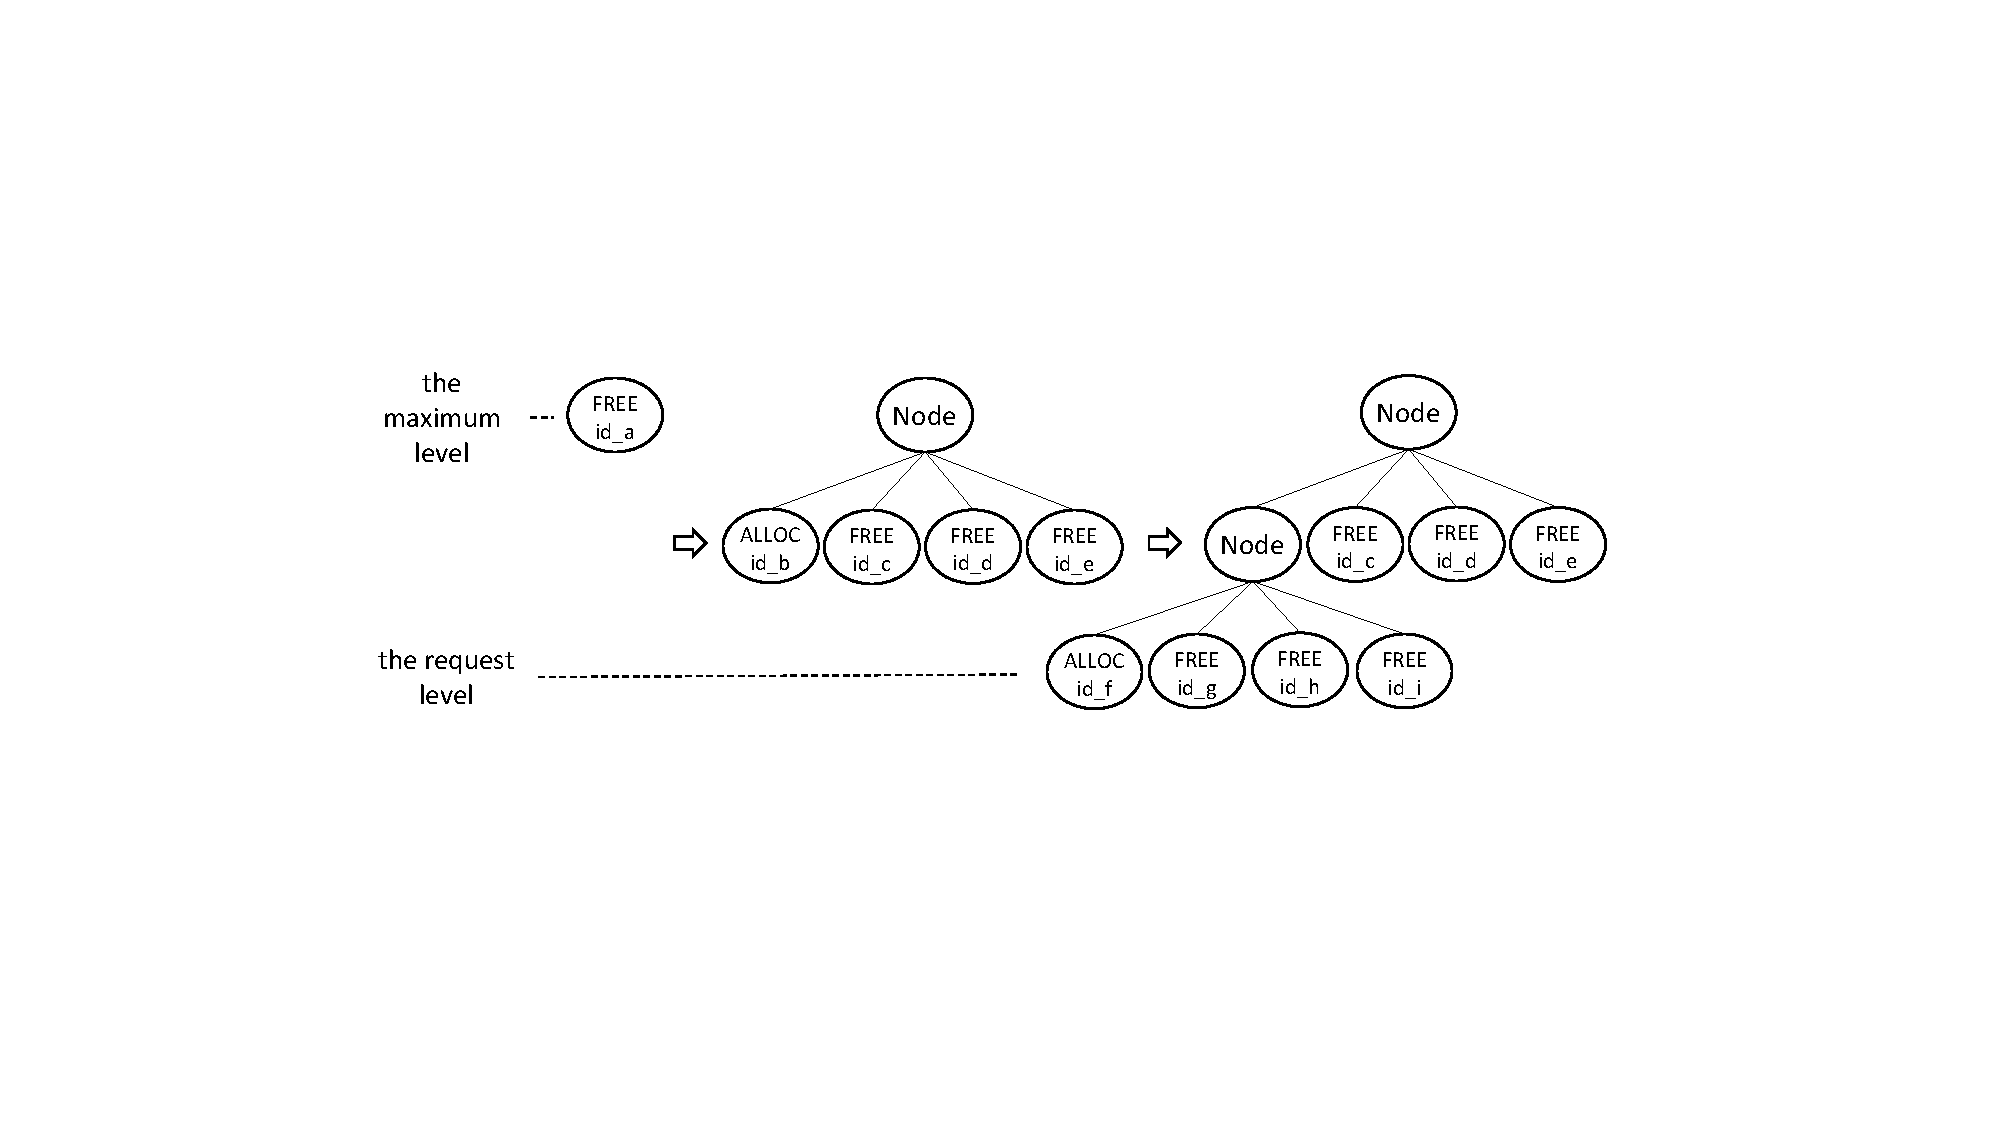
\includegraphics[width=1\textwidth]{fig1.pdf}
	\caption{The progress of dividing a free leaf}
	\label{fig1}
\end{figure*}

\begin{definition} [Split a Leaf Node]
\end{definition}
\vspace{-7pt}
{\footnotesize
\begin{align*}
split\ b\ lv \triangleq\ &if\ lv = 0\ then\ b \\
else\ Node\ &(split\ (LL\ divide\ b)\ (lv - 1))\ (LR\ divide\ b)\\ 
&(RL\ divide\ b)\ (RR\ divide\ b)
\end{align*}
}	
\vspace{-12pt}

In addition, we give functions \textbf{set\_type}, \textbf{replace} and \textbf{replace\_leaf} as follows: Function \emph{set\_type} takes a Leaf node \emph{b} and a target block\_state\_type \emph{s} as inputs, it changes the type of \emph{b} with \emph{s} as a new Leaf node \emph{b'}, finally it returns the new Leaf node \emph{b'}. Function \emph{replace} takes a Block \emph{btree}, two Leaf nodes \emph{b} and \emph{b'} as inputs, then it replaces the Leaf node \emph{b} with \emph{b'} in \emph{btree}, finally it returns the updated Block \emph{btree'}. Function \emph{replace\_leaf} takes a Block \emph{btree}, a Leaf node \emph{b} and a Node \emph{btr} as inputs, then it replaces the Leaf node \emph{b} with \emph{btr} in \emph{btree}, lastly it returns the updated Block \emph{btree'}.

Now we give the process of the allocation operation. It firstly checks whether there is a Block in \emph{bset} that has such \emph{FREE} Leaf nodes whose levels are less than or equal to \emph{rlv} by function \emph{exists\_freelevel}. If it returns \emph{False} then the allocation process stops and returns original \emph{bset} and \emph{False}. Otherwise, function \emph{freesets\_maxlevel} returns the maximum level \emph{lmax} among all levels with \emph{FREE} Leaf nodes but less than or equal to \emph{rlv}. Two branches are as follows.

If \emph{lmax} is equal to requested level \emph{rlv}, then the allocation operation randomly picks up such a Block tree as \emph{btree}, that has such \emph{FREE} Leaf nodes whose levels are equal to \emph{rlv}. After this, it randomly picks up a \emph{FREE} Leaf node \emph{l} in level \emph{rlv} from \emph{btree}. Then function \emph{set\_type} is invoked to set the type of \emph{l} as \emph{ALLOC}, and to return a new Leaf node \emph{l'}. Next, the opearation invokes function \emph{replace} to update \emph{btree} with \emph{l'}, and to return \emph{btree'}. After that, the allocation operation updates Block set \emph{bset} by replacing previous \emph{btree} with \emph{btree'}. Finally, the operation returns updated Block set and \emph{True}.

If \emph{lamx} is not equal to requested level \emph{rlv}, then the allocation operation randomly picks up such a Block tree as \emph{btree}, who has \emph{FREE} Leaf nodes in level \emph{lmax}. After that, it randomly picks up a \emph{FREE} Leaf node \emph{l} in level \emph{lmax} from \emph{btree}. Then function \emph{split} is invoked to split \emph{l} into Node tree \emph{btr}. Next, the operation invokes function \emph{replace\_leaf} to update \emph{btree} with \emph{btr}, and to return \emph{btree'}. After this, the allocation operation updates Block set \emph{bset} by replacing previous \emph{btree} with \emph{btree'}. Finally, the operation returns updated Block set and \emph{True}. The definition of allocation operation is as follows.

\begin{definition} [Allocation Operation]
\end{definition}
\vspace{-7pt}
{\footnotesize
\begin{align*}
alloc\ &bset\ rlv \triangleq \\
&if\ exists\_freelevel\ bset\ rlv\ then \\
&\ \ \ \ lmax = freesets\_maxlevel\ bset\ rlv \\
&\ \ \ \ if\ lmax = rlv\ then \\
&\ \ \ \ \ \ \ \ btree = SOME\ b.\ b \in bset \wedge freesets\_level\ b\ rlv \ne \emptyset \\
&\ \ \ \ \ \ \ \ l = SOME\ l.\ l \in freesets\_level\ btree\ rlv \\
&\ \ \ \ \ \ \ \ btree' = replace\ btree\ l\ (set\_type\ l\ ALLOC) \\
&\ \ \ \ \ \ \ \ return\ (bset - \lbrace btree \rbrace \cup \lbrace btree' \rbrace, True) \\
&\ \ \ \ else \\
&\ \ \ \ \ \ \ \ btree = SOME\ b.\ b \in bset \wedge freesets\_level\ b\ lmax \ne \emptyset \\
&\ \ \ \ \ \ \ \ l = SOME\ l.\ l \in freesets\_level\ btree\ lmax \\
&\ \ \ \ \ \ \ \ btr' = split\ l\ (rlv - lmax) \\
&\ \ \ \ \ \ \ \ btree' = replace\_leaf\ btree\ l\ btr' \\
&\ \ \ \ \ \ \ \ return\ (bset - \lbrace btree \rbrace \cup \lbrace btree' \rbrace, True) \\
&else\ return\ (bset, False)
\end{align*}
}
\vspace{-17pt}

\subsection{Deallocation Model}
During the deallocation process, if such a situation appears that four Leaf nodes belonging to a same parent Node are all \emph{FREE}, then function \textbf{merge} is invoked to merge these Leaf nodes to one Leaf node. It invokes function \textbf{combine} that takes a Node tree \emph{n} and returns a new terminal Leaf node \emph{l} \emph{iff} Node tree \emph{n} has four terminal \emph{FREE} Leaf nodes. Function \emph{merge} takes a Node tree \emph{n} and recursively invokes \emph{combine} on each sub-node of \emph{n} and \emph{n} itself. A simple example that describes the merging process is showed in Fig. \ref{fig2}.

\begin{figure*}[htbp]
	\centering
	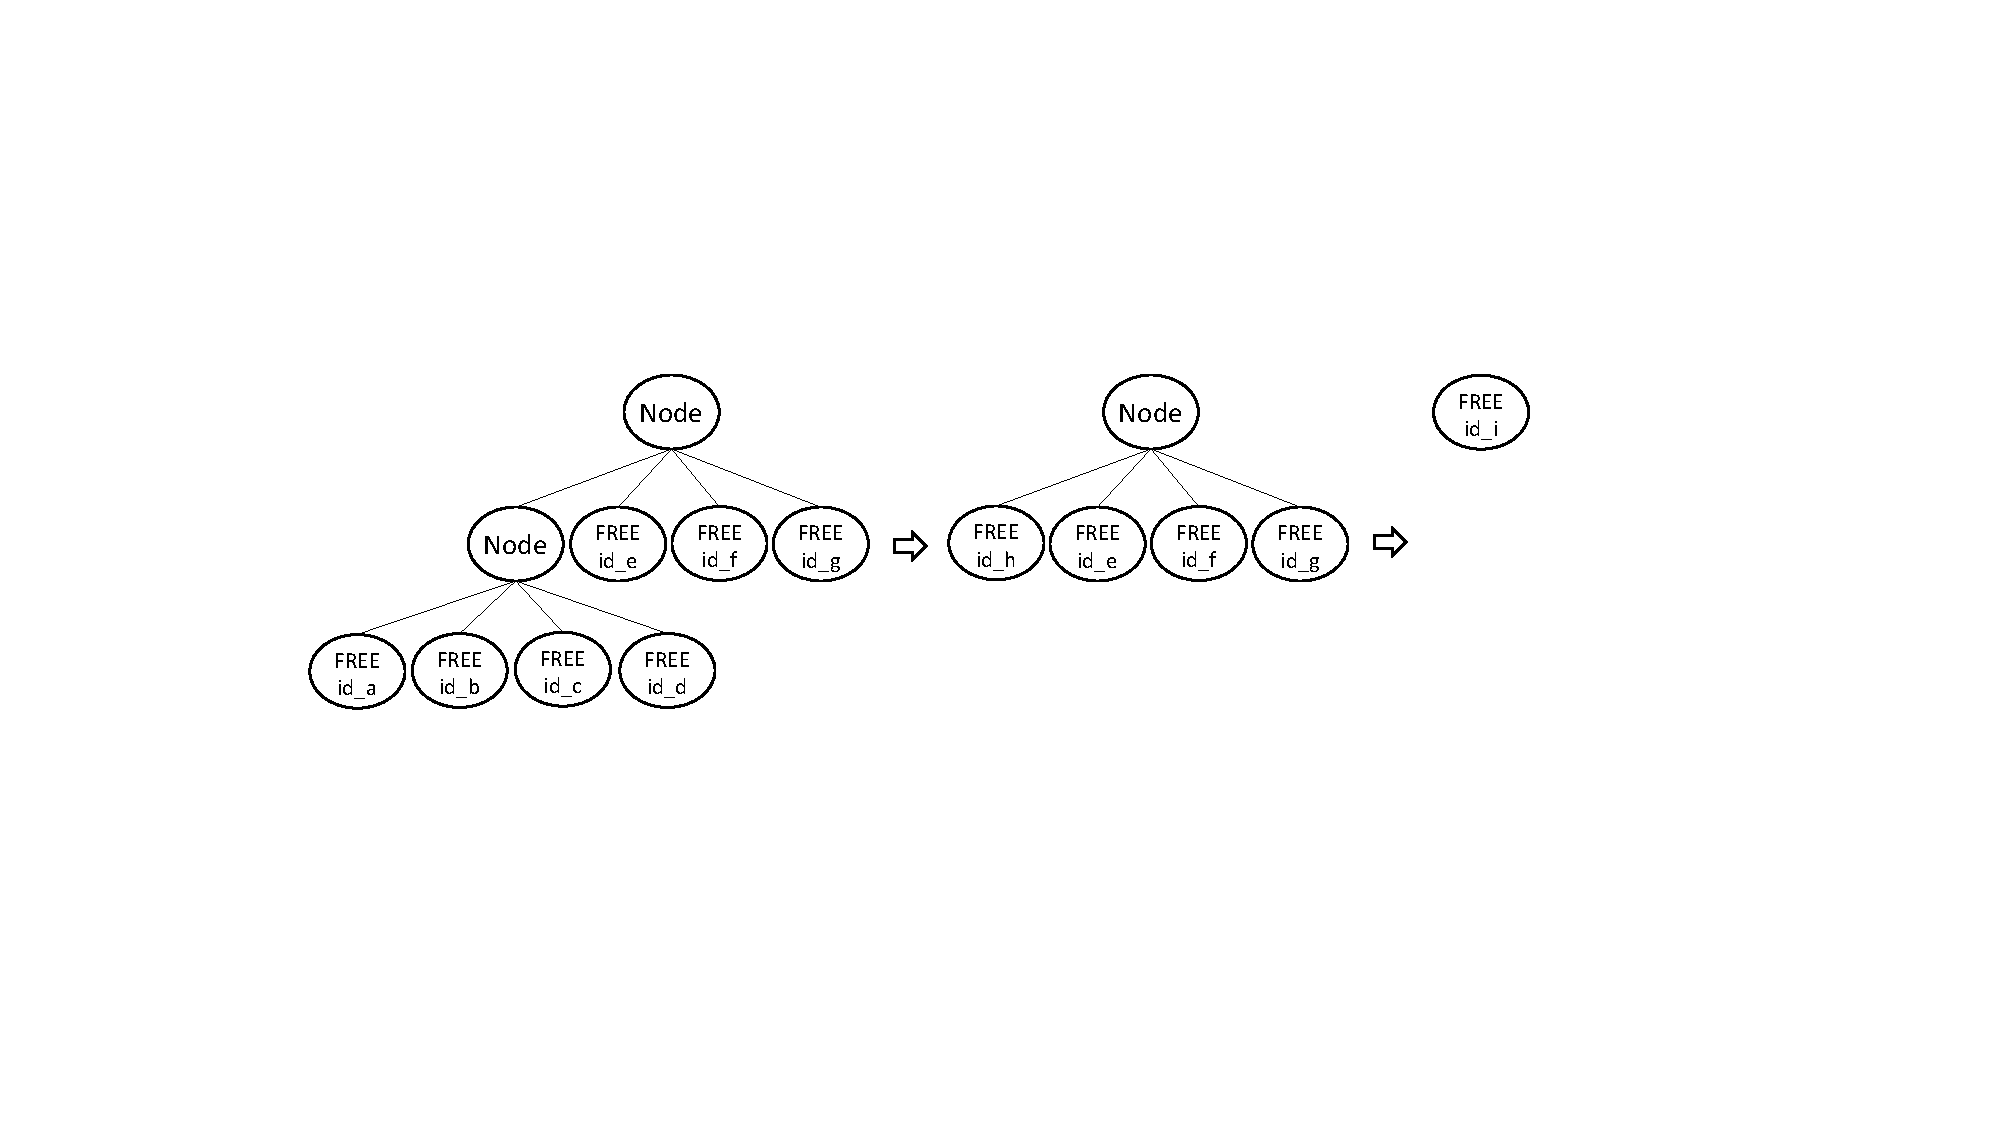
\includegraphics[width=1\textwidth]{fig2.pdf}
	\caption{The progress of merging all free memory blocks}
	\label{fig2}
\end{figure*}

With above discussion, we give the process of deallocation operation. It firstly checks whether there is a Block tree in \emph{bset} whom the Leaf node \emph{b} to be deposed belongs to. If there is no such tree, the procedure returns the original \emph{bset} and \emph{False}. Otherwise, if the type of \emph{b} is \emph{FREE}, it also returns the original \emph{bset} and \emph{False}. When all conditions are met, it picks up the Block tree in \emph{bset} as \emph{btree} whom \emph{b} belongs to. After this, the operation invokes function \emph{set\_type} to set the type of \emph{b} as \emph{FREE}, and to return a new Leaf node \emph{b'}. Next, it invokes function \emph{replace} to update \emph{btree} with \emph{b'}, and to return \emph{btree'}. After that, the deallocation operation invokes \emph{merge} to perform a necessary merging operation on \emph{btree'}, and to return \emph{btree''}. Next, the operation updates Block set \emph{bset} by replacing previous \emph{btree} with \emph{btree''}. Finally, the deallocation operation returns updated Block set and \emph{True}. The definition of deallocation operation is as follows.

\begin{definition} [Deallocation Operation]
\end{definition}
\vspace{-7pt}
{\footnotesize
\begin{align*}
free\ &bset\ b \triangleq \\
&if\ \exists btree \in bset.\ b \in set\ btree\ then \\
&\ \ \ \ if\ fst\ b = FREE\ then \\
&\ \ \ \ \ \ \ \ return\ (bset, False) \\
&\ \ \ \ else \\
&\ \ \ \ \ \ \ \ btree = THE\ t.\ t \in bset \wedge b \in set\ t \\
&\ \ \ \ \ \ \ \ btree' = replace\ btree\ b\ (set\_type\ b\ FREE) \\
&\ \ \ \ \ \ \ \ btree'' = merge\ btree' \\
&\ \ \ \ \ \ \ \ return\ (bset - \lbrace btree \rbrace \cup \lbrace btree'' \rbrace, True) \\
&else\ return\ (bset, False)
\end{align*}
}
\vspace{-12pt}

At this point, we have finished the specification for a buddy memory allocation algorithm. Next, we are going to verify its functional correctness and security property.